\section{Schaltungserweiterung mit ESP32}
Nachdem die Signalübertragung zwischen Lesegerät und Tag grundlegend gezeigt wurde, wird der Aufbau im nächsten Schritt um zwei ESP32 erweitert. Dabei geht es in diesem Kapitel noch nicht um den genauen Programmablauf, sondern nur um die notwendige Erweiterung der bestehenden Schaltungen.

Ein ESP32 wird beim Lesegerät platziert, der zweite ESP32 befindet sich auf der Tag-Seite. Dadurch sollen die bisher getrennt aufgebauten Modulations- und Demodulationsschaltungen später mit digitalen Signalen angesteuert und ausgewertet werden können.

\subsection{Erweiterung des Lesegeräts}
Auf der Seite des Lesegeräts wird der ESP32 als Steuer- und Auswerteeinheit vorgesehen. Sein digitales Ausgangssignal wird zur Ansteuerung der ASK-Stufe verwendet. Damit kann der ESP32 später festlegen, wann das Sendesignal aktiv ist und wann es abgeschaltet wird.

Zusätzlich wird ein Eingang für das empfangene beziehungsweise demodulierte Signal des Tags benötigt. Dieses Signal wird vom Lesegerät aus der Lastmodulation des Tags gewonnen und anschließ end dem ESP32 zugeführt.

Für die Anzeige der Leitungsaktivität werden zwei getrennte LED-Ausgänge eingeplant:

\begin{itemize}
  \item ein Ausgang für die TX-Aktivität des Lesegeräts,
  \item ein Ausgang für die RX-Aktivität des Lesegeräts.
\end{itemize}

Die geplante Schaltungserweiterung des Lesegeräts ist in \cref{fig:esp32_lesegeraet_platzhalter} dargestellt.

\begin{figure}[H]
  \centering
  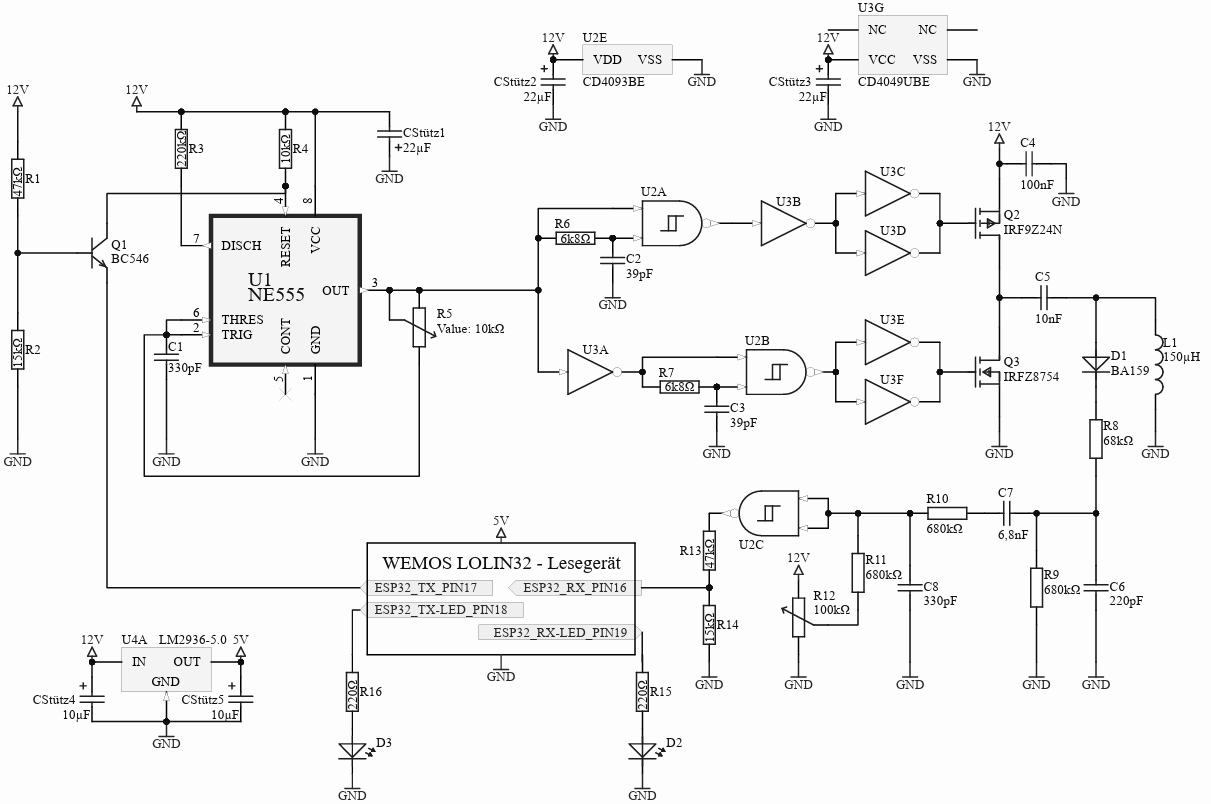
\includegraphics[width=0.8\linewidth]{Schaltungen/Lesegerät+ESP32.png}
  \caption{Geplante Schaltungserweiterung des Lesegeräts}
  \label{fig:esp32_lesegeraet_platzhalter}
\end{figure}

\subsection{Erweiterung des Tags}
Auf der Tag-Seite wird ebenfalls ein ESP32 in die Schaltung eingebunden. Er soll später die Modulationsstufe des Tags ansteuern und das vom Lesegerät kommende Signal auswerten. Da der Tag im eigentlichen Versuch vom Lesegerät versorgt werden soll, muss die Versorgung des ESP32 in die Tag-Schaltung integriert werden.

Wichtig ist dabei, dass der ESP32 auf der Tag-Seite erst dann aktiv wird, wenn die notwendige Versorgungsspannung vorhanden ist.

Auch beim Tag werden zwei LED-Ausgänge vorgesehen:

\begin{itemize}
  \item ein Ausgang für die TX-Aktivität des Tags,
  \item ein Ausgang für die RX-Aktivität des Tags.
\end{itemize}


Die geplante Schaltungserweiterung des Tags ist in \cref{fig:esp32_tag_platzhalter} dargestellt.

\begin{figure}[H]
  \centering
  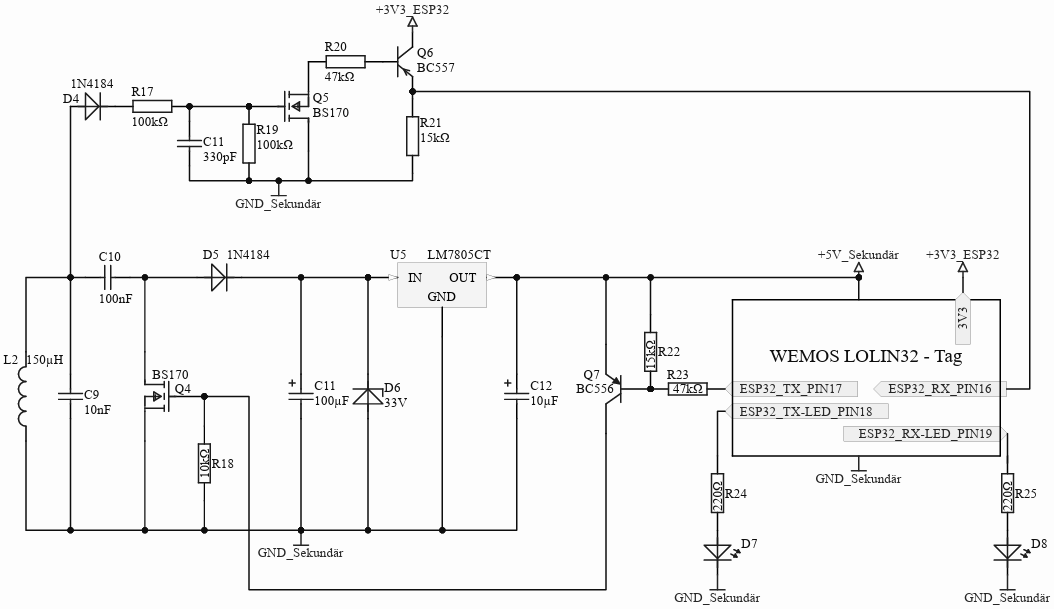
\includegraphics[width=0.8\linewidth]{Schaltungen/Tag+ESP32.png}
  \caption{Geplante Schaltungserweiterung des Tags}
  \label{fig:esp32_tag_platzhalter}
\end{figure}

\subsection{Signal- und Versorgungsschnittstellen}
Durch die Erweiterung entstehen auf beiden Seiten mehrere Schnittstellen zwischen analoger Schaltung und Mikrocontroller. Die wichtigsten Verbindungen sind die digitalen TX- und RX-Signale, die Ansteuerung der Modulationsstufe, das demodulierte Empfangssignal sowie die Versorgung des Tag-ESP32.

Die genaue Funktion der beiden ESP32, der Kommunikationsablauf und der experimentelle Testaufbau werden im folgenden Kapitel beschrieben.
